\documentclass[14pt]{beamer}
\usepackage[utf8]{inputenc}
\usepackage[utf8]{vietnam}
\usepackage{amsmath}
\usepackage{amsfonts}
\usepackage{amssymb}
\usepackage{graphicx}
\usepackage{xcolor}
\usepackage{tikz}
\usetikzlibrary{positioning}
\usepackage{utopia} %font utopia imported

\usepackage{ragged2e}
\usepackage{etoolbox}

\mode<beamer>{\usetheme{CambridgeUS}}

\usecolortheme{default}

\usepackage{hyperref}
\hypersetup{pdfpagemode=FullScreen} %mode FullScreen with beamer

\apptocmd{\frame}{}{\justifying}{} % Allow optional arguments after frame.

\usepackage{comment}

\makeatletter
\let\insertuniversity\relax
\newcommand\universitytitle{TRƯỜNG ĐH}

\let\insertclass\relax
\newcommand\classtitle{Lớp}

\let\insertcourse\relax
\newcommand\coursetitle{Môn học}

\mode<all>
{
  \newcommand\university[1]{\def\insertuniversity{#1}}
  
  \newcommand\class[1]{\def\insertclass{#1}}
  
  \newcommand\course[1]{\def\insertcourse{#1}}
  \titlegraphic{}
}

\defbeamertemplate*{title page}{supdefault}[1][]
{
  %\vbox{}
  %\vfill
  \begingroup
    \centering
    
    \ifx\insertuniversity\relax\relax\else
    \begin{beamercolorbox}[sep=4pt,center,#1]{author}
      %\usebeamerfont{institute}\universitytitle~\insertuniversity
      \small\universitytitle~\insertuniversity
    \end{beamercolorbox}\fi
    
    
    \begin{beamercolorbox}[sep=8pt,center,#1]{title}
      \usebeamerfont{title}\inserttitle\par%
      \ifx\insertsubtitle\@empty\relax%
      \else%
        \vskip0.25em%
        {\usebeamerfont{subtitle}\usebeamercolor[fg]{subtitle}\insertsubtitle\par}%
      \fi%     
    \end{beamercolorbox}%
    \vskip.5em\par
    
    \ifx\insertcourse\relax\relax\else
    \begin{beamercolorbox}[sep=6pt,center,#1]{author}
      \usebeamerfont{author}\coursetitle:~\insertcourse
    \end{beamercolorbox}\fi
    
    \ifx\insertclass\relax\relax\else
    \begin{beamercolorbox}[sep=6pt,center,#1]{author}
      \usebeamerfont{author}\classtitle:~\insertclass
    \end{beamercolorbox}\fi
    
    \begin{beamercolorbox}[sep=6pt,center,#1]{author}
      \usebeamerfont{author}\insertauthor
    \end{beamercolorbox}
    %\begin{beamercolorbox}[sep=8pt,center,#1]{institute}
      %\usebeamerfont{institute}\insertinstitute
    %\end{beamercolorbox}
    \begin{beamercolorbox}[sep=8pt,center,#1]{date}
      \usebeamerfont{date}\insertdate
    \end{beamercolorbox}\vskip0.5em
    {\usebeamercolor[fg]{titlegraphic}\inserttitlegraphic\par}
  \endgroup
  \vfill
}
\setbeamertemplate{title page}[supdefault][colsep=-4bp,rounded=true,shadow=\beamer@themerounded@shadow]\makeatother

%Title page
\title[Động cơ không đồng bộ]{\emph{Chủ đề báo cáo}\\ Điều khiển Công suất trượt trả về nguồn và Điều khiển động cơ dùng biến tần}
\author[Cơ sở Truyền động điện]{GVHD: Hồ Minh Nhị \and Nhóm SVTH: Nhóm 1}
\course{Cơ sở Truyền động điện}
\class{Công nghệ, kỹ thuật điện, điện tử}
\university{KỸ THUẬT -- CÔNG NGHỆ CẦN THƠ}
\date[Nhóm 1]{\today}
%\date[Nhóm 1]{Ngày 24 tháng 08 năm 2016}

%\logo{
\includegraphics[height=1.3cm]{logo_ctut.pdf}}

\definecolor{doden}{RGB}{204, 0, 0}
\newcommand{\giaithich}[1]{\textcolor{red}{$\longrightarrow$ #1}}
\newcommand{\noibat}[1]{\textcolor{red}{#1}}
\begin{document}
%http://tex.stackexchange.com/questions/82794/removing-page-number-from-title-frame-without-changing-the-theme
\bgroup
\makeatletter
\setbeamertemplate{footline}
{
  \leavevmode%
  \hbox{%
  \begin{beamercolorbox}[wd=.333333\paperwidth,ht=2.25ex,dp=1ex,center]{author in head/foot}%
    \usebeamerfont{author in head/foot}\insertshortauthor\expandafter\beamer@ifempty\expandafter{\beamer@shortinstitute}{}{~~(\insertshortinstitute)}
  \end{beamercolorbox}%
  \begin{beamercolorbox}[wd=.333333\paperwidth,ht=2.25ex,dp=1ex,center]{title in head/foot}%
    \usebeamerfont{title in head/foot}\insertshorttitle
  \end{beamercolorbox}%
  \begin{beamercolorbox}[wd=.333333\paperwidth,ht=2.25ex,dp=1ex,right]{date in head/foot}%
    \usebeamerfont{date in head/foot}\insertshortdate{}\hspace*{2em}
%    \insertframenumber{} / \inserttotalframenumber\hspace*{2ex} 
    \hspace*{6ex}
  \end{beamercolorbox}}%
  \vskip0pt%
}

\begin{frame}
\titlepage
\end{frame}
\egroup

\setcounter{framenumber}{0}

%--------------------------------------------------------------------------------
%--------------------------------------------------------------------------------
% Noi dung bao cao
\begin{frame}	%Trang muc luc
	\frametitle{Nội dung giải thích}
	\tableofcontents
\end{frame}

\section[Công suất trượt]{Điều khiển công suất trượt trả về nguồn}
\subsection*{ĐK dưới vận tốc đồng bộ}
\begin{frame}{ĐK công suất trượt}
		\begin{center}
			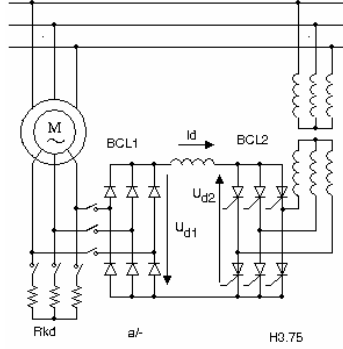
\includegraphics[scale=.4]{images-chude3/cascade-2.png} 
		\end{center}
		ĐK dưới vận tốc đồng bộ.\\
		\giaithich{$P_r$ qua bộ chỉnh lưu 1 $\longrightarrow$ nghịch lưu trả về nguồn.}
\end{frame}

\subsection*{ĐK trên vận tốc đồng bộ}
\begin{frame}{ĐK công suất trượt}
		\begin{center}
			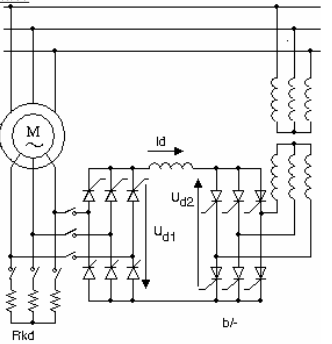
\includegraphics[scale=.4]{images-chude3/cascade.png} 
		\end{center}
		ĐK trên vận tốc đồng bộ.\\
		\giaithich{$P_r$ qua bộ chỉnh lưu 2 $\longrightarrow$ nghịch lưu đưa vào rotor.}
\end{frame}

%--------------------------------------------------------------------------------
%--------------------------------------------------------------------------------
\section[Biến tần]{Điều khiển động cơ dùng biến tần}
\subsection*{Khái quát}
\begin{frame}{Biến tần}{Khái quát}
	\begin{block}{Chức năng}	
		$U_1, I_1, f_1 \longrightarrow U_2, I_2, f_2$
		\giaithich{Thay đổi thông số ngõ vào.}
	\end{block}
	
	\begin{block}{Ứng dụng}
		\begin{itemize}
			\item Điều khiển tốc độ ĐC \giaithich{bằng pp tần số.}
			\item Thay đổi được số pha \giaithich{$1$ pha, $3$ pha, $m$ pha.}
		\end{itemize}
	\end{block}
\end{frame}

\begin{frame}{Biến tần}{Khái quát}
	\begin{block}{Phân loại}
		Theo \textcolor{blue}{cấu trúc}: biến tần \noibat{trực tiếp} và biến tần \noibat{gián tiếp}.
		\begin{itemize}
			\item Biến tần \noibat{trực tiếp}: \textcolor{blue}{không chứa} khâu trung gian một chiều.
			\item Biến tần \noibat{gián tiếp}: \textcolor{blue}{chứa} khâu trung gian một chiều.
		\end{itemize}
	\end{block}
\end{frame}

\subsection*{Cấu tạo}
\begin{frame}{Cấu tạo biến tần}
	\vspace{-1.5cm}
	\begin{flushleft}
		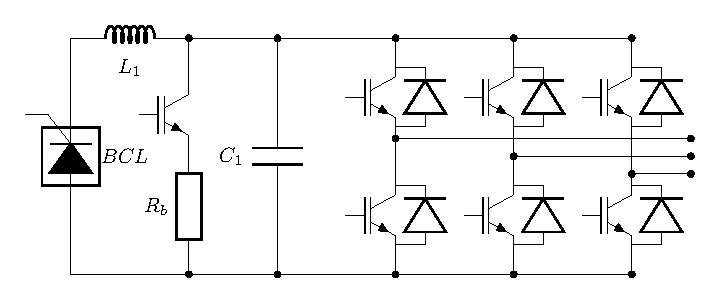
\includegraphics[scale=1]{images-chude3/bientan.pdf}
	\end{flushleft}
	\giaithich{Gồm 2 phần chính: bộ chỉnh lưu và bộ nghịch lưu.}\\
	\giaithich{$L_1, C_1$: nắn dòng điện và điện áp chỉnh lưu.}
\end{frame}

\begin{frame}{Cấu tạo biến tần}
	\begin{itemize}
		\item Bộ chỉnh lưu \giaithich{1 pha hoặc 3 pha.}
		\item Mạch trung gian (nếu có).
		\item Bộ nghịch lưu\giaithich{mạch tia, mạch cầu 1 pha, 3 pha.}
	\end{itemize}
	\giaithich{Chỉnh lưu 1 pha, nghịch lưu 3 pha: biến tần thay đổi được số pha.}
\end{frame}
\end{document}